% =============================================================
%  Chapitre 2 — Analyse et spécification des besoins
% =============================================================
\chapter{Analyse et spécification des besoins}

\section{Introduction}

Ce chapitre détaille les besoins de l'application Telnet Test Manager.
On commence par identifier les acteurs du système, puis on passe aux
besoins fonctionnels et non fonctionnels. Le diagramme des cas
d'utilisation et les scénarios principaux complètent cette analyse.

% -----------------------------------------------------------------
\section{Identification des acteurs}
% -----------------------------------------------------------------

\subsection{Administrateur}

L'\textbf{Administrateur} a accès à toutes les fonctionnalités du
système. Il gère les comptes utilisateurs, configure les équipements,
consulte les journaux d'audit et suit les tests et rapports générés.

\subsection{Technicien}

Le \textbf{Technicien} est le principal utilisateur terrain. Son rôle
se limite à lancer des tests Telnet sur les équipements configurés,
consulter les résultats en temps réel et générer des rapports.

\subsection{Ingénieur}

L'\textbf{Ingénieur} s'occupe de la configuration des équipements et
de la bibliothèque de commandes Telnet. Il pilote les campagnes de
tests, analyse les résultats et produit des rapports. Il dispose de
tous les droits du Technicien, en plus des siens.

% -----------------------------------------------------------------
\section{Besoins fonctionnels}
% -----------------------------------------------------------------

\begin{table}[H]
  \centering
  \caption{Récapitulatif des besoins fonctionnels}
  \label{tab:besoins_fonctionnels}
  \begin{tabular}{|C{1cm}|L{3cm}|L{9.5cm}|}
    \hline
    \textbf{ID} & \textbf{Module} & \textbf{Description} \\
    \hline
    BF-01 & Authentification &
      Connexion JWT, RBAC (3 rôles), limitation de débit \\
    \hline
    BF-02 & Équipements &
      CRUD complet~: Poste / Produit / Slot / Référence \\
    \hline
    BF-03 & Commandes &
      Bibliothèque~: single, séquence, monitoring \\
    \hline
    BF-04 & Tests Telnet &
      Exécution, validation de réponse, arrêt à la demande \\
    \hline
    BF-05 & Multi-slots &
      Lancement parallèle via Worker Threads isolés \\
    \hline
    BF-06 & Temps réel &
      Diffusion des événements de test via WebSocket \\
    \hline
    BF-07 & Rapports &
      Compilation, filtrage, statistiques de campagne \\
    \hline
    BF-08 & Administration &
      Gestion utilisateurs, journal d'audit, analytiques \\
    \hline
    BF-09 & Monitoring &
      Métriques Prometheus, dashboards Grafana, alertes \\
    \hline
  \end{tabular}
\end{table}

% -----------------------------------------------------------------
\section{Besoins non fonctionnels}
% -----------------------------------------------------------------

\begin{table}[H]
  \centering
  \caption{Contraintes techniques et non fonctionnelles}
  \label{tab:besoins_non_fonctionnels}
  \begin{tabular}{|L{3cm}|L{4.5cm}|L{6cm}|}
    \hline
    \textbf{Catégorie} & \textbf{Exigence} & \textbf{Critère de mesure} \\
    \hline
    \multirow{2}{*}{\textbf{Performance}}
      & Temps de réponse API & 95\,\% des requêtes $<$ 2\,s \\
    \cline{2-3}
      & Parallélisme & 10 tests Telnet simultanés minimum \\
    \hline
    \multirow{3}{*}{\textbf{Sécurité}}
      & Authentification & JWT HS256, expiration configurable \\
    \cline{2-3}
      & Mots de passe & bcryptjs, coût~: 10 \\
    \cline{2-3}
      & En-têtes HTTP & Helmet.js~: CSP, HSTS, X-Frame \\
    \hline
    \textbf{Disponibilité}
      & Objectif de service & 99,9\,\% sur l'infrastructure locale \\
    \hline
    \multirow{2}{*}{\textbf{Scalabilité}}
      & Autoscaling & HPA~: 1--5 répliques, seuil CPU 70\,\% \\
    \cline{2-3}
      & Sans état & Backend stateless, session JWT \\
    \hline
    \textbf{Maintenabilité}
      & Architecture & Clean Architecture, principes SOLID \\
    \hline
    \textbf{Portabilité}
      & Conteneurisation & Images Docker identiques dev/production \\
    \hline
  \end{tabular}
\end{table}

% -----------------------------------------------------------------
\section{Diagramme des cas d'utilisation}
% -----------------------------------------------------------------

\begin{figure}[H]
  \centering
  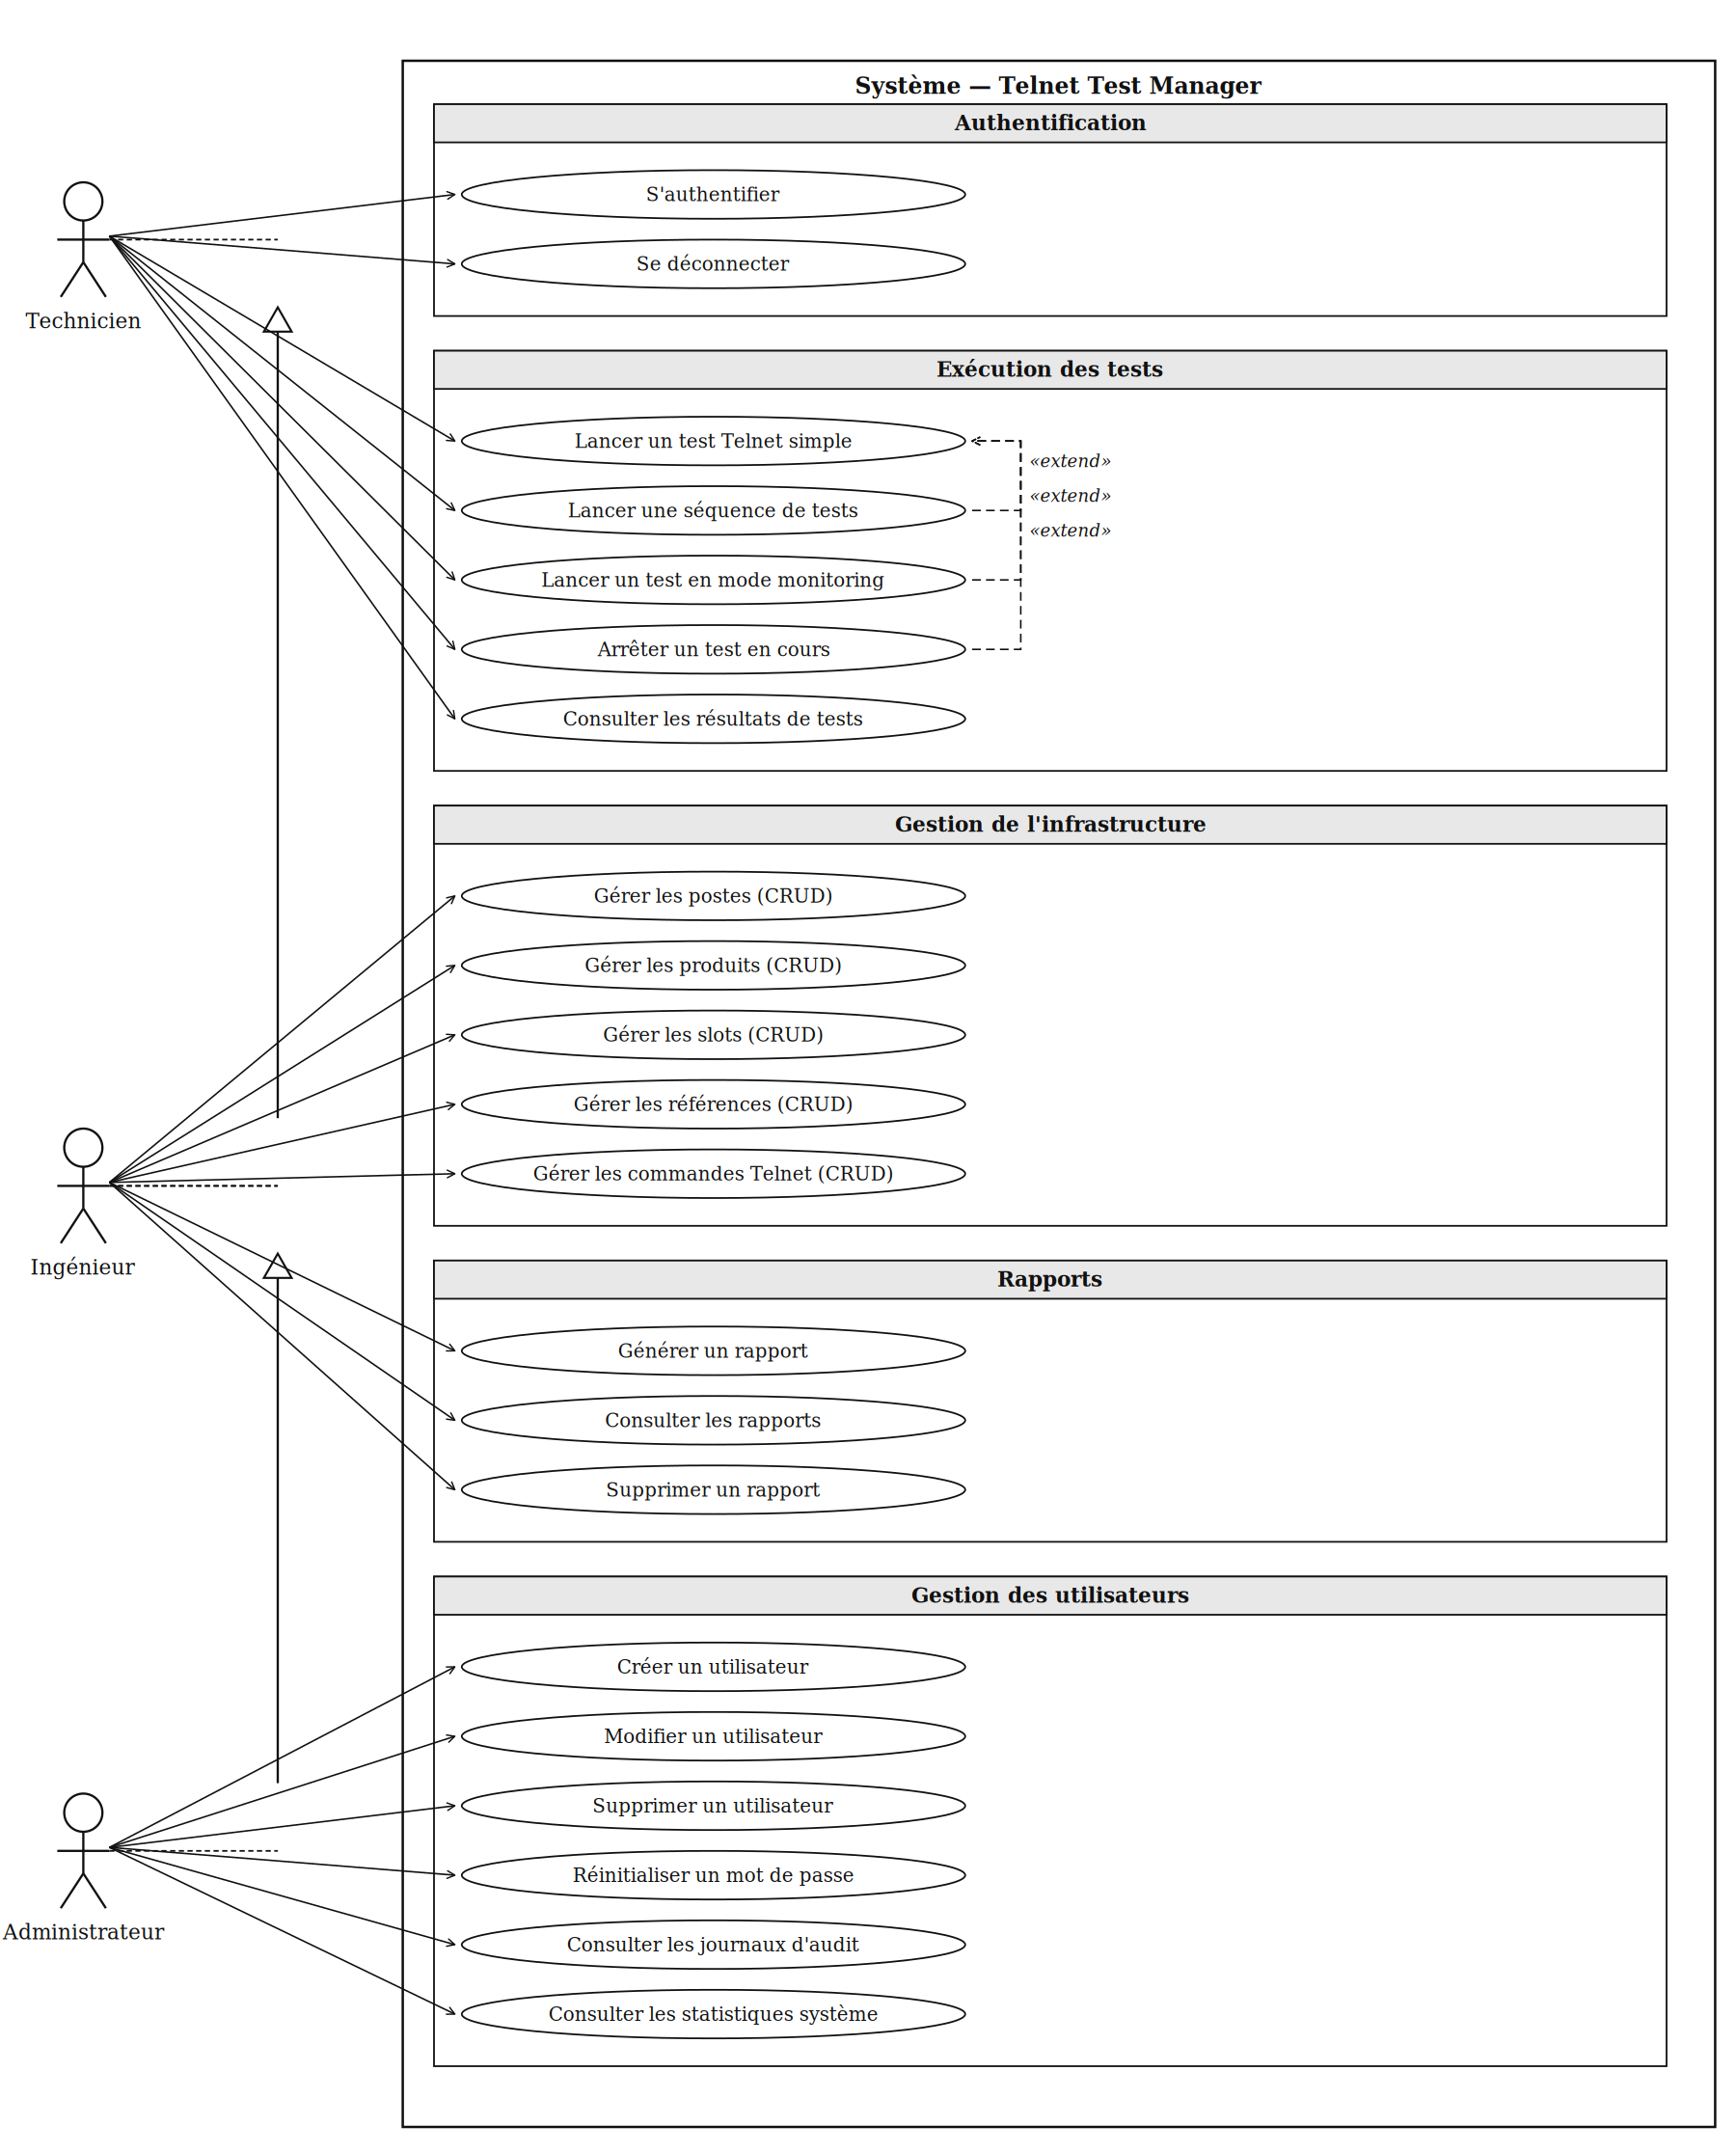
\includegraphics[width=\textwidth]{images/usecase_diagram}
  \caption{Diagramme des cas d'utilisation global --- Telnet Test Manager}
  \label{fig:usecase}
\end{figure}

% -----------------------------------------------------------------
\section{Description des cas d'utilisation principaux}
% -----------------------------------------------------------------

\begin{table}[H]
  \centering
  \caption{UC-01 --- S'authentifier}
  \label{tab:uc01}
  \begin{tabular}{|L{3.5cm}|L{10cm}|}
    \hline
    \textbf{Nom} & S'authentifier \\
    \hline
    \textbf{Acteurs} & Technicien, Ingénieur, Administrateur \\
    \hline
    \textbf{Préconditions} & L'utilisateur dispose d'un compte actif en base \\
    \hline
    \textbf{Postconditions} & Un jeton JWT est généré et stocké côté client \\
    \hline
    \textbf{Scénario nominal} &
      1.~L'acteur saisit son identifiant et son mot de passe \\
    & 2.~Le système vérifie les identifiants et le statut du compte \\
    & 3.~Le système génère un JWT signé HS256 \\
    & 4.~Le frontend stocke le token et redirige vers le Dashboard \\
    \hline
    \textbf{Alternatives} &
      A1.~Identifiants incorrects~: 401 «~Identifiants invalides~» \\
    & A2.~Compte inactif~: 401 «~Compte inactif~» \\
    & A3.~10 tentatives échouées~: 429, blocage 15\,min \\
    \hline
  \end{tabular}
\end{table}

\begin{table}[H]
  \centering
  \caption{UC-04 --- Lancer un test Telnet}
  \label{tab:uc04}
  \begin{tabular}{|L{3.5cm}|L{10cm}|}
    \hline
    \textbf{Nom} & Lancer un test Telnet \\
    \hline
    \textbf{Acteurs} & Technicien, Ingénieur \\
    \hline
    \textbf{Préconditions} & Utilisateur authentifié, slot configuré et équipement accessible \\
    \hline
    \textbf{Postconditions} & Résultat enregistré en base (SUCCESS, FAIL ou STOPPED) \\
    \hline
    \textbf{Scénario nominal} &
      1.~L'acteur sélectionne Poste, Produit, Slot et la commande \\
    & 2.~L'acteur clique «~Lancer le test~» \\
    & 3.~Le backend crée un résultat PENDING et spawne un Worker Thread \\
    & 4.~Le Worker établit la connexion TCP port 23 \\
    & 5.~Le Worker exécute la commande et valide la réponse \\
    & 6.~Chaque étape est diffusée en temps réel via WebSocket \\
    & 7.~Le résultat final est enregistré en MongoDB \\
    \hline
    \textbf{Alternatives} &
      A1.~Connexion TCP impossible~: timeout, statut FAIL \\
    & A2.~Réponse incorrecte~: sous-chaîne attendue absente, FAIL \\
    & A3.~L'acteur arrête le test~: \texttt{POST /stop-test}, statut STOPPED \\
    \hline
  \end{tabular}
\end{table}

\begin{table}[H]
  \centering
  \caption{UC-07 --- Générer un rapport}
  \label{tab:uc07}
  \begin{tabular}{|L{3.5cm}|L{10cm}|}
    \hline
    \textbf{Nom} & Générer un rapport \\
    \hline
    \textbf{Acteurs} & Technicien, Ingénieur, Administrateur \\
    \hline
    \textbf{Préconditions} & Des résultats de tests existent en base \\
    \hline
    \textbf{Postconditions} & Un rapport de synthèse est enregistré et affiché \\
    \hline
    \textbf{Scénario nominal} &
      1.~L'acteur applique des filtres (date, statut, slot) \\
    & 2.~Le frontend envoie POST /reports/generate \\
    & 3.~Le backend récupère les résultats filtrés depuis MongoDB \\
    & 4.~Le backend calcule taux de succès, durée moyenne, total \\
    & 5.~Le rapport est enregistré et retourné (201) \\
    & 6.~Le frontend affiche le rapport de synthèse \\
    \hline
    \textbf{Alternatives} &
      A1.~Aucun résultat ne correspond aux filtres~: 404 \\
    \hline
  \end{tabular}
\end{table}

\section{Conclusion}

Ce chapitre a permis de cadrer les besoins de Telnet Test Manager.
Les trois acteurs --- Administrateur, Ingénieur et Technicien ---
couvrent tous les rôles du système. Les neuf besoins fonctionnels
organisés par module couvrent le cycle complet des tests Telnet,
de la connexion à la génération des rapports. Les besoins non
fonctionnels fixent les contraintes de performance, sécurité,
scalabilité et disponibilité. Le chapitre suivant aborde la
conception et les choix architecturaux retenus.
